\chapter{Electrical Power System}
\label{chap:eps}

\section{Introduction}
\label{sec:introduction}

The \ac{EPS} provides power to motors, the on-board computer, communication system and payloads. Power is mainly supplied from solar cells but can also be supplied from a battery, when solar power is not available or insufficient. 

\enlargethispage{2.0em}

\subsection{Changes from PDR to CDR}
\label{sec:changes_pdr_to_cdr}
%
Table \ref{tab:pdr_to_cdr} lists major design changes from the \ac{EPS} \ac{PDR} report.

\begin{table}[H]
\centering
\caption{Design changes from PDR to CDR}
\label{tab:pdr_to_cdr}
\begin{tabular}{p{0.25\textwidth}p{0.3\textwidth}p{0.4\textwidth}}
\hline
\textbf{Area of change} & \textbf{Changed parameter } & \textbf{Argumentation for change}\\
\hline
Total power budget & Increased to $>40\,W$ & Airship total mass and size are increased thus requiring much more power for the motors\\
Solar cells & New part & Old solar cell was much heavier than listed in manufacturer datasheet due to a glass cover\\
Total system cost & Increased to $>12000\,SEK$ & Increased power and new light-weight solar cells are more expensive\\
Solar cell mounting & New part & New solar cell is flexible instead of rigid and can be mounted with \ac{PSA}\\
Battery & New part & A battery that supports much higher discharge currents has been selected which simplifies current limiting circuitry and improves battery efficiency\\
\hline
\end{tabular}
\end{table} 
%
%
\section{Functional and Technical Requirements}
\label{sec:requirements}
This section describes the functional and technical \ac{EPS} requirements along with the expected \ac{EPS} performance.
%
\subsection{Functional Requirements}
The primary functional \ac{EPS} requirements are:
%
\begin{itemize}
\item Provide adequate power to motors, other subsystems and payloads
\item Proof that flying on solar energy is possible i.e more power produced than consumed
\end{itemize}
%
Additional desired requirements are:
%
\begin{itemize}
\item Scalable and flexible system architecture allowing the \ac{EPS} to be upgraded to higher power levels or re-used in different applications (rover, \ac{UAV} etc.)
\item Robust design allowing flight in more extreme conditions (altitude, weather etc.)
\item Provide adequate protection circuits for battery and loads to prevent any major failure and damage to other subsystem components.
\item Optimal design and high performance to increase power capability and minimize system mass
\end{itemize}
%
\subsection{Technical Requirements}
The \ac{EPS} technical requirements are listed in table \ref{tab:technical_requirements}.
%
\begin{table}[H]
\centering
\caption{Technical requirements}
\label{tab:technical_requirements}
\begin{minipage}{\textwidth}
\begin{tabular}{p{0.35\textwidth}p{0.15\textwidth}p{0.4\textwidth}}
\hline
\textbf{Description} & \textbf{Symbol} & \textbf{Value}\\
\hline
Minimum power output & $P_{out,min}$ & $40\,W$\footnote{Average \ac{SAR} output power including losses}\\
Maximum mass & $W_{EPS,max}$ & $1000\,g$ including solar arrays\\
Maximum cost & - & $4000\,SEK$\footnote{Initial budget for 2 students}\\
Output voltages & $V_{mainbus}$, $V_{5V}$ & $6.0-9.5\,V$ un-regulated and $5\,V$ regulated\\
Operational temperature & $T_{min}$, $T_{max}$ & $-20^{\circ}C\,to +45^{\circ}C$\\
Battery capacity & $C_{bat}$ & $>5\,Wh$\\
\hline
\end{tabular}\par
\vspace{-0.75\skip\footins}
\renewcommand{\footnoterule}{}
\end{minipage}
\end{table}

\subsection{Mission and Environmental Constraints}
\label{subsec:environmental_requirements}
This section discusses the system challenges imposed by the operation environment.

\subsubsection*{Solar Array Temperature}
As was discussed in \cite{PDR}, the optimal operating voltage of the solar cells change with temperature. The \ac{EPS} must be able to generate optimal power from the solar cells in the full expected temperature range of the environment. This can be achieved using a \ac{MPPTU} which will be discussed in Section \ref{sec:MPPTU}

\subsubsection*{Solar Incidence Angle}
The flight location of U-SPACE is near Kiruna in Sweden. Figure \ref{fig:SolarIncidenceAngles} shows the average solar incidence angles in Kiruna for the months June and September\cite{web:solarincidence}, considering a flat solar panel facing straight up.
The solar cell output current drops with the Kelly cosine function as shown in figure \ref{fig:KellyCosine}. To minimize power losses due to inclined solar incidence, \ac{MSE} design must consider the optimal mounting position and angle of the solar panels. The most optimal flight conditions are at noon in June, with a solar incidence angle of around $46^{\circ}$, however that still reduces the solar array output by about $30\%$. If the solar array output should not drop by more than $50\%$, the maximum solar incidence angle is about $57^{\circ}$. This is only an approximation from the assumption that the solar array is mounted flat on top of the airship envelope, which will not be the exact case in practical.
%
\begin{figure}[H]
\centering
\begin{minipage}[t]{0.48\linewidth}
\centering
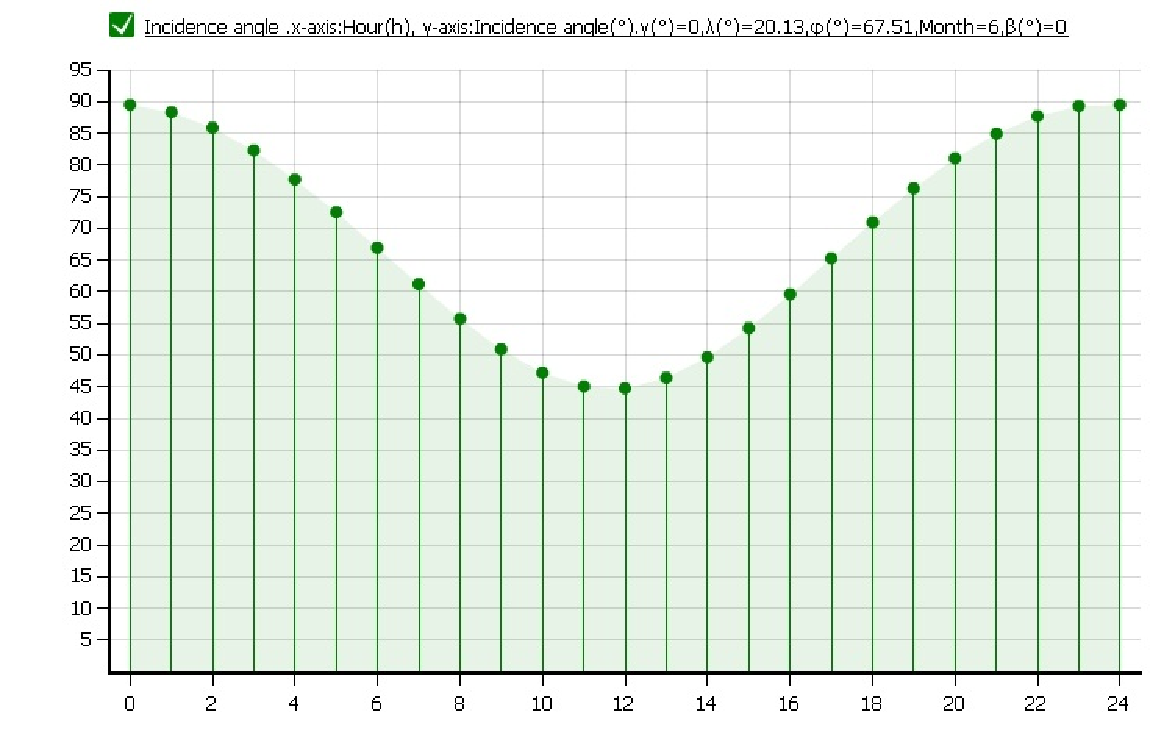
\includegraphics[width=\textwidth]{figures/fig_CDR_EPS_SolarIncidenceAngle_Jun}
\end{minipage}
%\vspace{0.5mm}
\begin{minipage}[t]{0.48\linewidth}
\centering
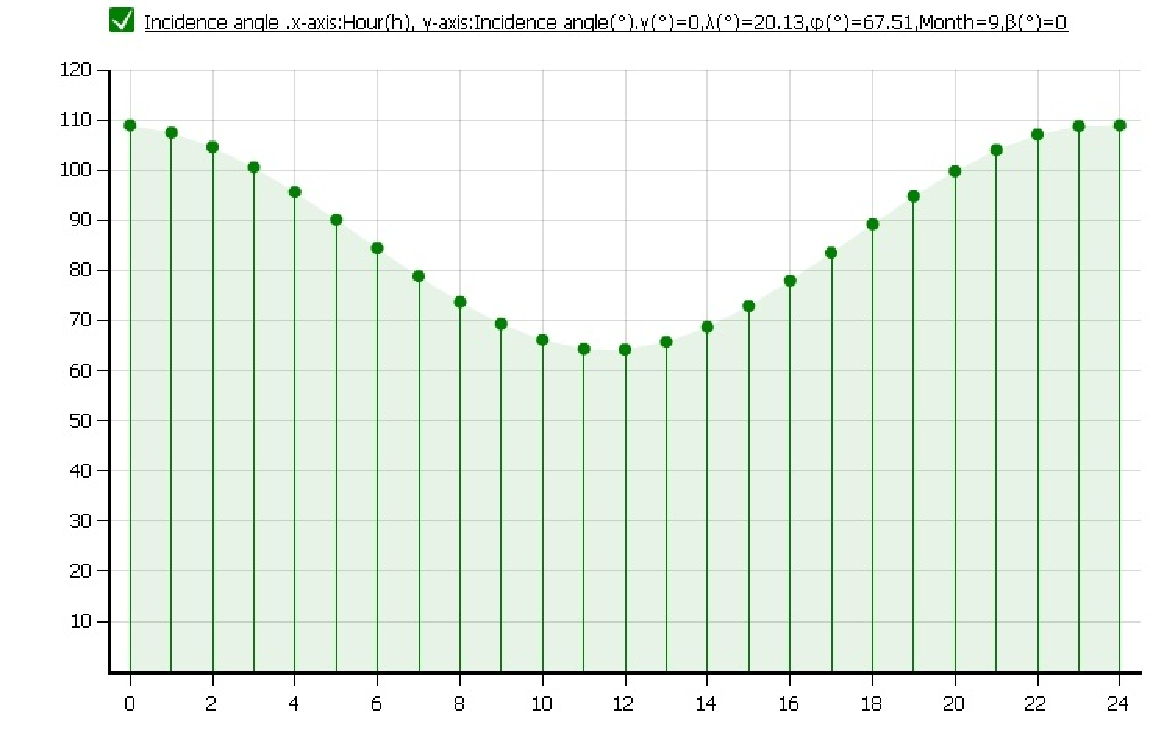
\includegraphics[width=\textwidth]{figures/fig_CDR_EPS_SolarIncidenceAngle_Sep}
\end{minipage}
\caption[Solar Incidence Angles]{Monthly average solar incidence angles for June(left) and September(right) for each hour of the day. Solar panel is facing straight up}
\label{fig:SolarIncidenceAngles}
\end{figure}
%
\begin{figure}[H]
\centering
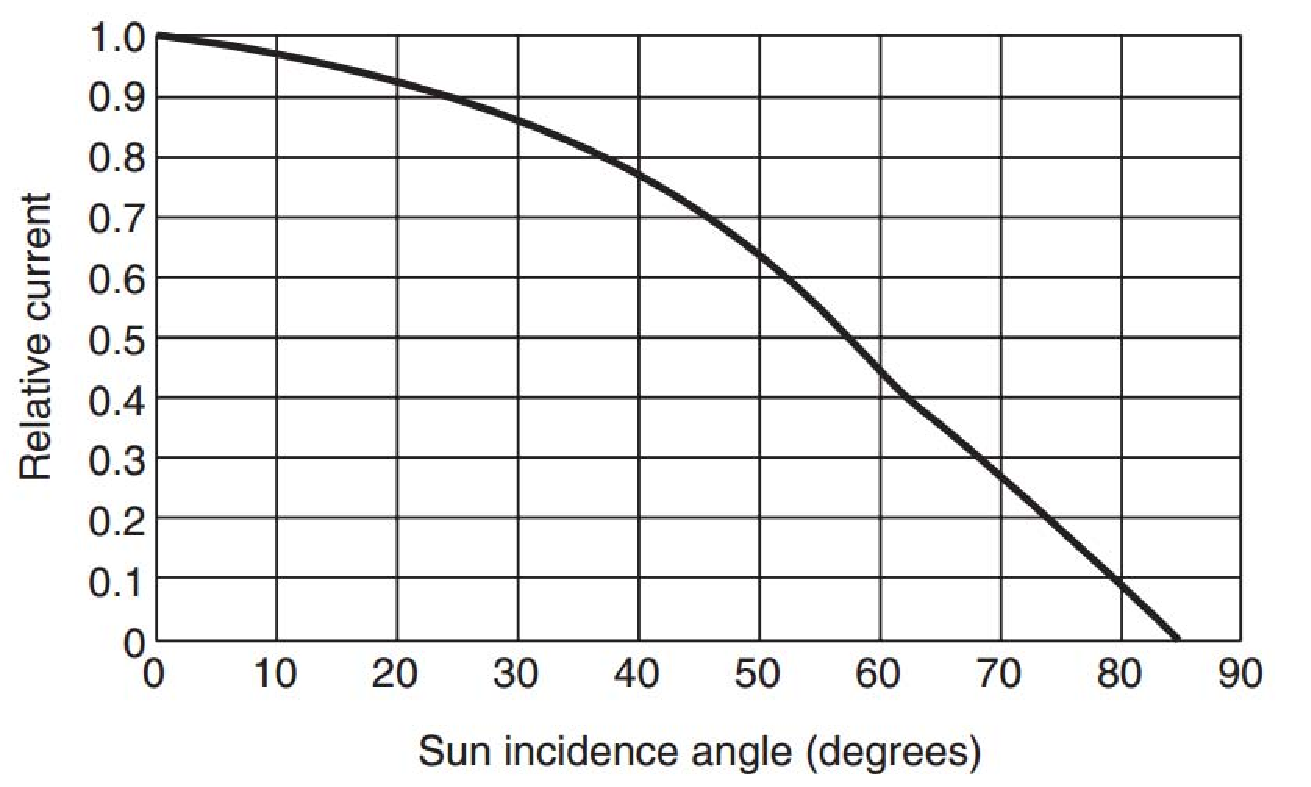
\includegraphics[scale=0.4]{figures/fig_KellyCosine}
\caption[Kelly cosine function]{Kelly cosine function showing how solar cell photo current depends on sun incidence angle\cite[Fig 9.12]{book:mukund_wind}}
\label{fig:KellyCosine}
\end{figure}
%
%
\subsubsection*{Solar Array Shading}
Shading on the solar panels, for example caused by airship stabilizer structures or objects in the landscape, can cause a significant drop in the cell output voltage, as described in \cite[p. 165]{Mukund}. Bypass diodes can be used to partly mitigate this issue. However, since the airship is only expected to fly at altitudes above terrain and buildings the only shading possibly expected is from the airship structure hence the \ac{MSE} design must consider this restriction.
%
\subsubsection*{Battery Temperature}
One of the most temperature critical \ac{EPS} components is the battery which must stay within its safety temperature limits. In the proposed design, only temperature monitoring is offered therefore, flight is only allowed when outdoors temperatures are well within the allowed battery temperature range. Otherwise a battery heater and more sophisticated thermal design may be necessary.
%
\subsection{Expected Performance}
The expected \ac{EPS} performance values are listed in Table \ref{tab:expected_performance}.
%
\begin{table}[H]
\centering
\caption{Expected performance}
\label{tab:expected_performance}
\begin{minipage}{\textwidth}
\begin{tabular}{p{0.4\textwidth}p{0.15\textwidth}p{0.35\textwidth}}
\hline
\textbf{Description} & \textbf{Symbol} & \textbf{Value}\\
\hline
Power conversion efficiency(SAR) & - & $>90\%$\\
Power output(SAR) & $P_{out}$ & $\sim 45\,W$\footnote{For ideal weather conditions, i.e. no clouds and best expected solar incidence angle}\\
Battery capacity & $C_{bat}$ & $7.3\,Wh$\\
Mass & $W_{EPS}$ & $\sim980\,g$\\
Total cost & - & $\sim12000\,SEK$\footnote{Solar cells are significantly more expensive than anticipated. A request for more funds is under preparation.}\\
\hline
\end{tabular}\par
\vspace{-0.75\skip\footins}
\renewcommand{\footnoterule}{}
\end{minipage}
\end{table}
%
%
\section{Critical Design}
\label{sec:critical_design}
%
The basic \ac{EPS} diagram is shown in  Figure \ref{fig:EPS_diagram_simple}. A \ac{SAR} controls the operating voltage of the solar array and supplies an unregulated mainbus. The mainbus voltage is mainly controlled by the battery voltage. A DC-DC regulator provides a regulated $5\,V$ supply to subsystems and payloads. Motors are supplied from the unregulated mainbus.
%
\begin{figure}[H]
\centering
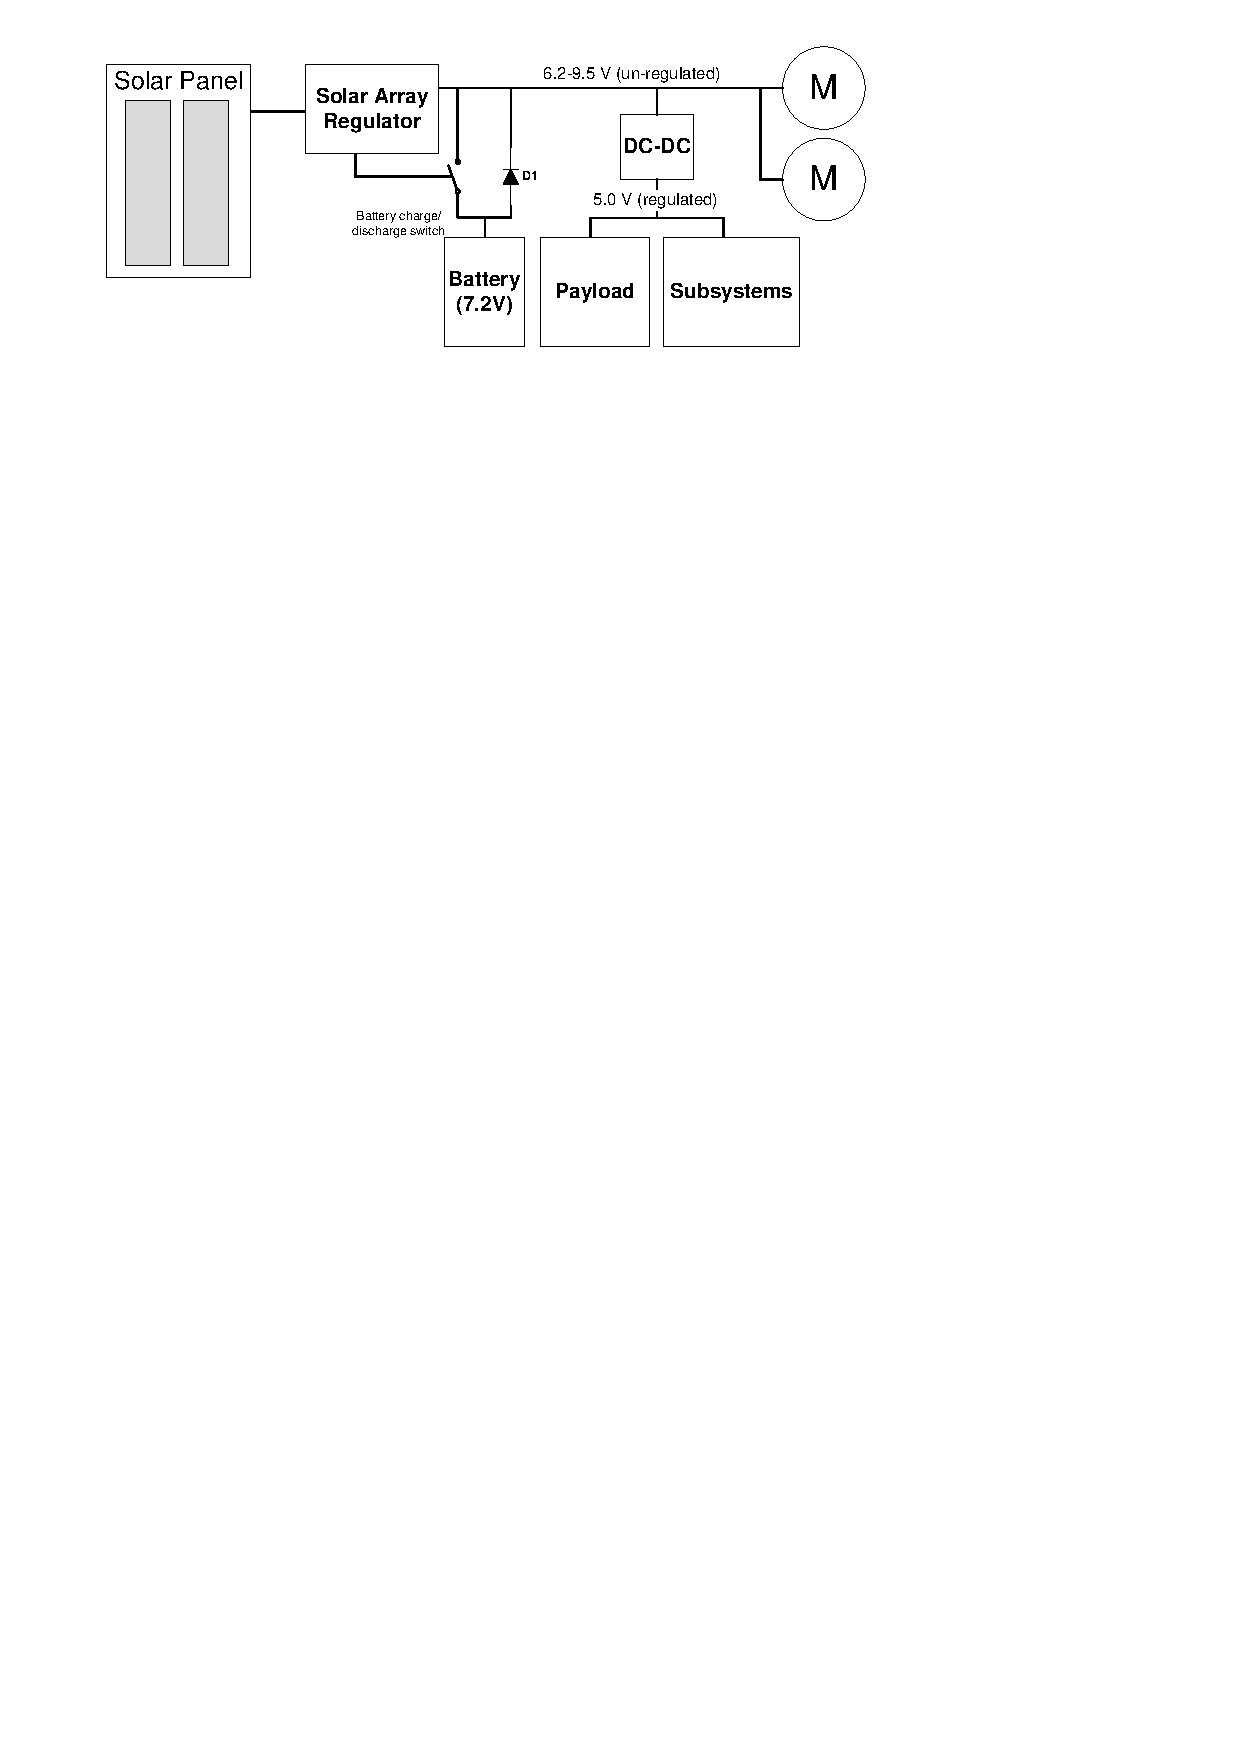
\includegraphics[width=\textwidth]{figures/fig_PDR_EPSdiagram}
\caption{EPS simple block diagram}
\label{fig:EPS_diagram_simple}
\end{figure}
%
%
\subsection{Battery Design}
In \cite{PDR} it was decided that a Li-ion type battery was suitable for the \ac{EPS}. An \textit{Ansmann \ac{LiPo} Racing Pack 2S1P 30C} battery is selected with the specifications as listed in Table \ref{tab:proposed_battery}.
%
\begin{table}[H]
\centering
\caption{Specification of chosen battery}
\label{tab:proposed_battery}
\begin{tabular}{p{0.35\textwidth}p{0.15\textwidth}p{0.4\textwidth}}
\hline
\textbf{Description} & \textbf{Symbol} & \textbf{Value}\\
\hline 
Chemistry & - & Li-Polymer\\
Nominal voltage & $V_{bat}$ & $7.4\,V$\\
Capacity & $C_{bat}$ & $2.1\,Ah$ / $15.54\,Wh$\\
Weight & $W_{bat}$ & $122\,g$\\
Dimensions & - & $105\,mm\:\times\:35.2\,mm\:\times\:17\,mm$\\
Maximum fast charge current & $I_{charge,max}$ & $3\,A$\\
Maximum discharge current (continuous) & $I_{discharge,max}$ & $63\,A$\\
\hline
\end{tabular}
\end{table}
%
%
\subsubsection{Battery Charge Regulator}
\label{subsec:BCR}
%
The \ac{BCR} must control the charge rate of the battery such that the charge current limit is not exceeded and cut off the charge current when the battery is fully charged. Temperature monitoring is usually also required to inhibit charging if the battery temperature is outside its safety limits. 

\pagebreak

\noindent
An \textit{MCP73842} Li-ion battery charge regulator \ac{IC} is selected. It employs three different charge modes: low-charge for deeply discharged batteries, \ac{CC} charge and trickle charging as well as inputs for temperature monitoring. The battery maximum charge current was in Table \ref{tab:proposed_battery} given as $3\,A$. From the \textit{MCP73842} datasheet, the minimum current sense resistor value is calculated as
%
\begin{equation}
\begin{split}
R_{sense}=&\dfrac{V_{FCS}}{I_{REG}}\\
R_{sense}=&\dfrac{120\,mV}{3\,A}=40\,m\Omega
\end{split}
\end{equation}
%
A $50\,m \Omega$ current sense resistor is selected leading to a charge current of $2.4\,A$.
%
The worst-case thermal dissipation in the MOSFET happens when the battery is charged from its minimum charge state
%
\begin{equation}
\footnotesize{P_{max,MOSFET}=(V_{in,max}-V_F-V_{bat,min})\cdot I_{charge}=(9.5\,V-0.3\,V-5.5\,V)\cdot 2.4\,A=8.88\,W}
\end{equation}
%
where $V_{in,max}$ is the maximum mainbus voltage, $V_F$ the expected Schottky diode forward voltage drop and $V_{bat,min}$ is the preconditioning threshold voltage of the \ac{BCR} \ac{IC}.
An \textit{SUP75P03-07-E3} P-channel MOSFET is selected which is rated for a peak power dissipation of $187\,W$, well above the minimum requirement provided that suitable thermal design is applied, most likely also including a heat sink. 
\\
\\
Calculations on heat sink requirements still remain to be done.
%
\subsubsection*{Future Improvements}
As was calculated above, significant power may be lost in the \ac{BCR} MOSFET. This is due to the selected \ac{BCR} \ac{IC} which requires an input voltage of around $9.5\,V$ (including a Schottky diode forward voltage drop and some design margin). In future, the \ac{BCR} could be designed to allow operation with an input voltage only slightly above the battery voltage thus minimizing the charge losses and the thermal requirements of the MOSFET.
%
%
\subsubsection{Battery Temperature Monitoring}
%%
The selected \ac{LiPo} battery is rated, in charge-mode, for the temperature interval $0$ to $+45^{\circ}C$. For temperature measuring, a $4.7\,k \Omega$ \textit{NTCLE203E3472GB0} thermistor is selected which has a Beta Value, $B=3977\,K$. Since the battery temperature is measured using an external thermistor, thus the temperature response is likely to be somewhat slower, an extra $5^{\circ}C$ thermal design margin is added. The required resistance values of the \ac{BCR} temperature control resistors are determined from the \textit{MCP73842} datasheet as 
%
\begin{equation}
\begin{split}
R_{cold}&=R_{25}\,e^{B(\dfrac{1}{T}-\dfrac{1}{T_0})}=4.7\,k\Omega \,e^{3977\,K(\dfrac{1}{278	\,K}-\dfrac{1}{298\,K})}=12.28\,k\Omega\\
R_{hot}&=4.7\,k\Omega \, e^{3977\,K(\dfrac{1}{313	\,K}-\dfrac{1}{298\,K})}=2.48\,k\Omega\\
R_{T1}&=2\dfrac{R_{cold}R_{hot}}{R_{cold}-R_{hot}}=6.2\,k\Omega\\
R_{T2}&=2\dfrac{R_{cold}R_{hot}}{R_{cold}-3R_{hot}}=12.6\,k\Omega
\end{split}
\end{equation}
%
where $R_{25}$, $R_{cold}$ and $R_{hot}$ are the thermistor resistance values at room temperature, the low and high temperature limits respectively. $R_{T1}$ and $R_{T2}$ are the required \ac{BCR} temperature control resistors setting the required temperature interval.
\\
\\
If the sensed battery temperature falls outside the $+5$ to $+40^{\circ}\,C$ region, battery charging will be inhibited. The technical requirements from Table \ref{tab:technical_requirements} requires the \ac{EPS} to operate down to $-20^{\circ}\,C$. Hence some insulation and/or heating of the battery may be necessary or flight must be disallowed at outdoors temperatures much below $+5^{\circ}\,C$.
%
\subsubsection{Battery Under-Voltage Lock-Out}
To prevent over-discharge of the battery, a battery \ac{UVLO} circuit is added as shown in Figure \ref{fig:EPS_diagram_detailed}. An \textit{TL431} precision shunt regulator \ac{IC} is selected. The lock-out voltage is given as
%
\begin{equation}
V_{UVLO}=V_{ref}(1+\dfrac{R_1}{R_2})=2.5\,V(1+\dfrac{29\,k \Omega}{20\,k \Omega})=6.125\,V
\end{equation}
%
where $V_{ref}$ is the \textit{TL431} build-in voltage reference. If the battery voltage drops below this value, the gate voltage to the P-type MOSFET is pulled high thus opening the switch. The $1\,M \Omega$ resistor adds about $200\,mV$ hysteresis. 
\\
\\
The \ac{UVLO} circuit only cuts out the motor power line. Thus payloads remain supplied and the battery is still slowly drained. This design has been chosen to allow  telemetry and telecommand capability during a heavy battery discharge event. In this case, it is expected that all payloads and on-board computers enter a low power consumption mode, to extend the remaining battery supply time. If the battery voltage drops below $5.62\,V$, the $5\,V$ payload power supply shuts down and all telemetry and telecommand capabilities will be lost.

\pagebreak

\subsection{Solar Array Design}
\label{sec:SA}
The main driver for selecting the solar cell is to choose a part which is very light-weight and easy to mount on the \ac{SPA}. A  \textit{PowerFilm RC7.2-75(PSA)} solar cell is selected as shown in Figure \ref{fig:solar_cell}. This is a very light-weight flexible solar cell with a \ac{PSA} backside for mounting. Table \ref{tab:solar_cell_spec} lists the solar cell specifications.
%
\begin{table}[H]
\centering
\caption{Specifications of chosen solar cell}
\label{tab:solar_cell_spec}
\begin{minipage}{\textwidth}
\begin{tabular}{p{0.35\textwidth}p{0.15\textwidth}p{0.4\textwidth}}
\hline
\textbf{Description} & \textbf{Symbol} & \textbf{Value}\\
\hline
Nominal output current & $I_{cell}$ & $100\,mA$\\
Nominal output voltage & $V_{cell}$ & $7.2V$\\
Nominal output power & $P_{cell}$ & $0.72\,W$\\
Dimensions & - & $270\,mm\:\times\:90\,mm\:\times\:0.2\,mm$\\
Weight & $W_{cell}$ & $7.6\,g$\\
No. of required cells & $N_{cells}$ & $100$\footnote{\cite{avnetexpress} offers good discount for +100 units order}\\
Total solar array area & $A_{array}$ & $2.43\,m^2$ (assuming $100\,\%$ fill factor)\\
\hline
\end{tabular}\par
\vspace{-0.75\skip\footins}
\renewcommand{\footnoterule}{}
\end{minipage}
\end{table}

\noindent
The solar array is an array of 50 parallel connected strings of two series solar cells as shown in Figure \ref{fig:solar_cell}. The nominal output voltage and current are given as
%
\begin{equation}
\begin{split}
V_{array}&=2\cdot V_{cell}=14.4\,V\\
I_{array}&=50\cdot I_{cell}=5\,A
\end{split}
\end{equation}
%
\begin{figure}[H]
\centering
\begin{minipage}[t]{0.4\linewidth}
\centering
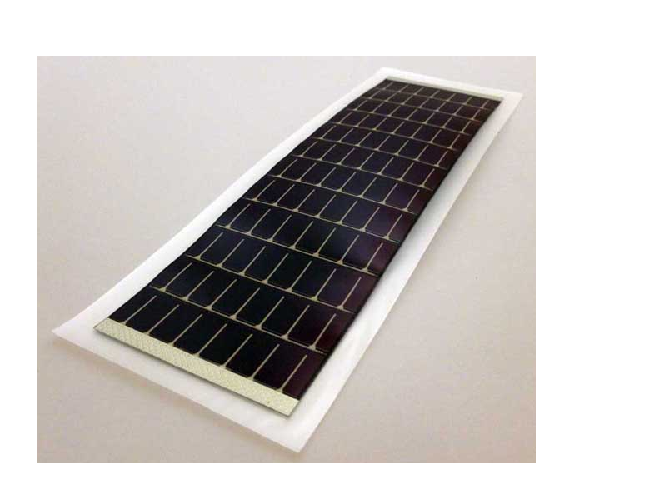
\includegraphics[width=\textwidth]{figures/SolarCell_RC7-2_Powerfilm}
\end{minipage}
\hspace{5mm}
\begin{minipage}[t]{0.55\linewidth}
\centering
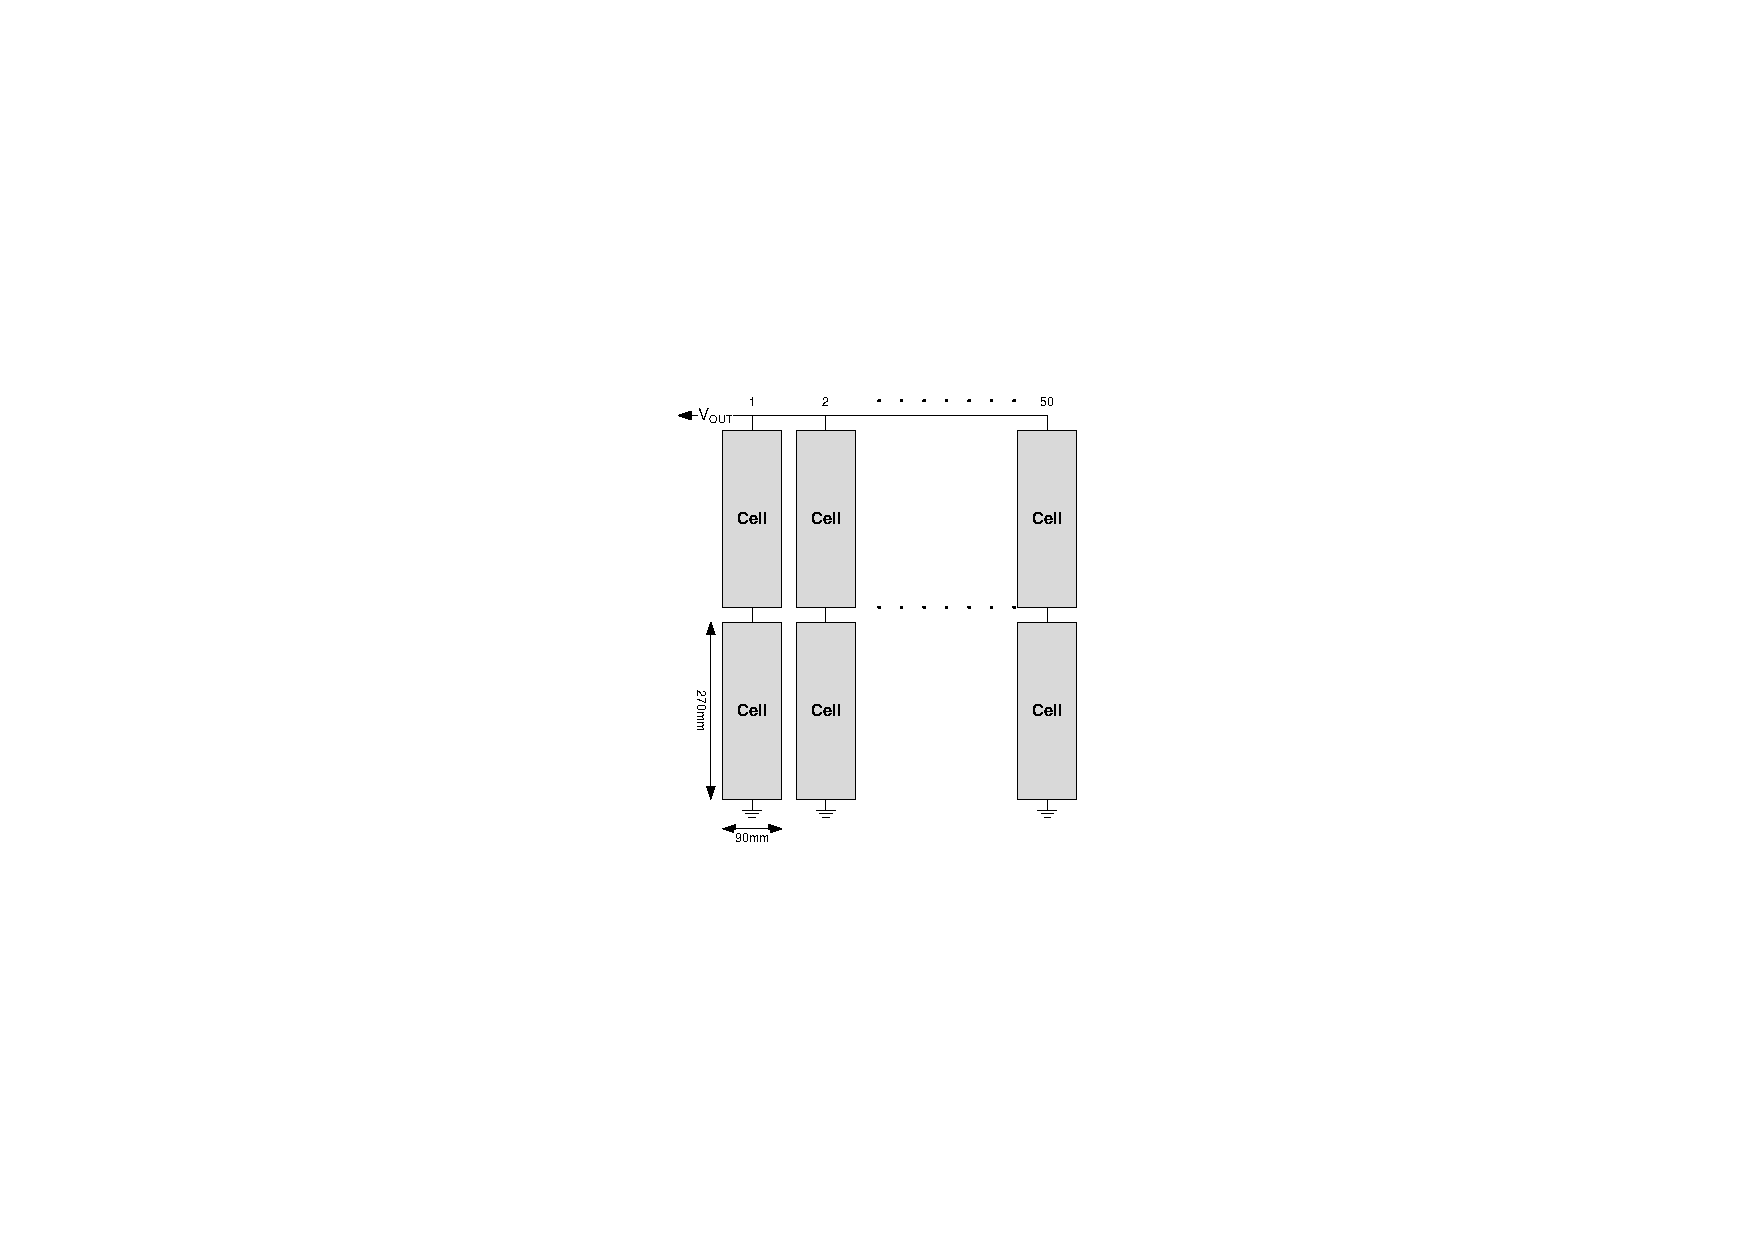
\includegraphics[width=0.9\textwidth]{figures/fig_CDR_Solar_Array}
\end{minipage}
\caption{PowerFilm solar cell (left) and solar array configuration (right)}
\label{fig:solar_cell}
\end{figure}
%
\noindent
Since only two cells are in series, it is estimated that bypass diodes are not very beneficial for mitigating shading issues, as was discussed in Section \ref{subsec:environmental_requirements}, and hence are not included in the design.
%
\subsection{Solar Array Regulator}
The \ac{SAR} must control the optimal the solar array operating voltage as well as limit the output mainbus voltage. A simple step-down buck converter topology is preferred for a number of reasons:
%
\begin{itemize}
\item simple circuit analysis and low components count
\item no inherent \ac{RHPZ} in contrary to the standard boost topology
\item step-down topology calls for a high input voltage which leads to low input current thus minimizing ohmic losses and the relative forward voltage drop loss from the reverse protection diode
\end{itemize}
%
\subsubsection{Buck Converter Circuit Design}
The ideal transfer function for the buck converter shown in Figure \ref{fig:EPS_diagram_detailed} is given as
%
\begin{equation}
V_{out}=D\,V_{in}
\end{equation}
%
where $D$ is the duty cycle of the MOSFET switch, $V_{in}$ the solar array voltage and $V_{out}$ the mainbus voltage. The duty cycle is controlled by a \ac{PWM} controller which provides input to a high-side MOSFET driver. A \ac{MEA} measures the mainbus output voltage to generate a control signal for the PWM controller. An \textit{LM3477} chip is selected which combines \ac{PWM} controller, \ac{MEA} and gate driver in one \ac{IC}.
\\
\\
The \ac{CM} control scheme is adopted due to its excellent dynamic abilities\cite[sec. 12-3-6]{Fundamentals} and simplified feedback regulator design. A low resistance $10\,m \Omega$ precision sense resistor measures the inductor current slope. The \textit{LM3477} has build-in slope compensation to avoid current mode instabilities\cite[sec. 12-1]{Fundamentals}.
\\
\\
The converter switching frequency, $f_{switch}$, is chosen relatively high to $500\,kHz$. The increased switching losses are expected to by out-weighted by the fact that the low operating voltage limits switching losses and high frequency allows the inductor and filter components to be made smaller thus limiting system mass and the resistive losses in the inductor copper wires which are expected to dominate converter losses due to the relatively high currents.

\noindent
The inductor current ripple, $\Delta I_L$, can be calculated as 
%
\begin{equation}
\Delta I_L=\dfrac{V_{in}-V_{out}}{L\,f_{switch}}D
\end{equation}
%
where $L$ is the inductance and $f_{switch}$ the converter switching frequency. 
The inductor current ripple is usually limited to about $10\,\%$ of the maximum converter output current leading to a minimum required inductance of
%
\begin{equation}
L=\dfrac{V_{in}-V_{out}}{\Delta I_L\,f_{switch}}D=\dfrac{14.4\,V-7.4\,V}{10\% \cdot 10.83\,A\cdot 500\,kHz}\cdot 0.514=6.7\,uH
\end{equation}
%
where $10.83\,A$ is the maximum converter output current calculated as 
%
\begin{equation}
I_{SAR,max}=\dfrac{P_{out,max}}{V_{out,min}}=\dfrac{65\,W}{6.0\,V}=10.83\,A
\end{equation}
%
A $10\,uH$ inductor is chosen giving a current ripple of about $0.72\,A$. If the load current drops below $0.36\,A$, which is unlikely to happen in most operating modes, the converter will enter \ac{DCM}.
\\
\\
For the converter output capacitor, a component is chosen which has very low \ac{ESR} and high capacitance to limit the output voltage ripples.
%
\subsubsection*{Current Sense Amplifier}
With an inductor current ripple of $0.72\,A$ the current sense voltage slope is only 
%
\begin{equation}
v_{sense}=\Delta I_L\cdot R_{sense}=0.72\,A\cdot 10\,m\Omega = 7.2\,mV
\end{equation}
%
It is recommended that the slope compensation is equal to or the double of the sense slope\cite[sec. 12-1]{Fundamentals}, however the minimum compensation slope is limited to $103\,mV$ by the \textit{LM3477} chip. Thus the sensed slope signal must be amplified with a gain of around 20 being suitable. This also has the advantage of eliminating some of the typical noise susceptibility in the current sense signal. The current sense circuit in Figure \ref{fig:EPS_diagram_detailed} consists of two differential OpAmps which amplifies the current sense slope. Resistive voltage dividers are placed on the OpAmp inputs to scale down the input voltage signals to always be below the $5\,V$ OpAmp supply voltage.

Since a closed-loop OpAmp gain of 20 is needed at an operating frequency of $500\,kHz$, the gain-bandwidth specification of the OpAmps must be more than $10\,MHz$. The \textit{LTC6362CMS8PBF} OpAmp is chosen. One limitation of this OpAmp is its temperature range which only goes down to $0^{\circ}\,C$. This might be solved by thermally connecting it to the transistor heat sinks or ensure that the internal \ac{EPS} temperature does not go below $0^{\circ}\,C$.
%
\subsubsection*{Input Filter}
An input filter is placed in front of the buck converter, mainly to draw a continuous current from the solar array. It also reduces the converter \ac{EMC} issues. 
One challenge with the input filter is that it effects the dynamic properties of the converter and if not properly designed, it can degrade the control feedback loop performance. A damping network in the filter is also necessary to avoid instabilities\cite[sec. 10-3]{Fundamentals}.
\\
\\
A usable filter has been designed based on PSpice simulations. However thorough analysis still remains to be done to optimize the filter design.
%
%
\subsubsection{Maximum Power Point Tracker Unit}
\label{sec:MPPTU}
In \cite{PDR} it was decided to use a \ac{MPPTU} with the \ac{SAR} to increase solar array efficiency during changing environment conditions.
%
The \ac{SAR} with \ac{MPPT} can operate in three different operation regions:
%
\begin{itemize}
\item Battery discharge - when the solar array input power is insufficient to cover the load power demand, the battery is slowly discharged in order to maintain the output voltage. The \ac{MPPTU} controls the input solar array voltage.
\item Battery charge - when the solar array input is greater than the load power, excessive power is used to recharge the battery. The \ac{MPPTU} controls the input solar array voltage.
\item Input power limitation - when the battery is fully charged, the regulator will operate the solar array at a non-optimal voltage, thus limiting the input power to keep the output voltage at a maximum limit. The extra potential input power is dissipated as heat externally on the solar arrays.
\end{itemize}
%
It is preferred to implement an analog \ac{MPPTU} mainly since this makes the circuit independent on a control signal from a more complicated external \ac{MCU} or \ac{DSP} thus allowing a flexible plug'n-play system to be implemented. One challenge with an analog \ac{MPPTU} is the typical need for expensive analog multipliers\cite{Liang}. Since the required multiplier only needs to be a 1st quadrant type (only two positive inputs), it is believed that a low-cost multiplier can be build using standard discrete components\cite{Multiplier}.
%
\\
\\
The \ac{MPPTU} design still remains to be completed.
%
%
\subsubsection{Mode Transitions}
%
As was discussed in Section \ref{sec:MPPTU}, the \ac{SAR} can operate in three different main modes. The transition between the modes is controlled by the mainbus output voltage as shown in Figure \ref{fig:SAR_ModeTransition}. If the \ac{SAR} input power is lower than the load power, the battery will discharge and the mainbus voltage will follow the battery voltage. Once the input power is larger than the load power, the mainbus capacitor will quickly be charged to a voltage higher than the battery voltage. Once the mainbus capacitor voltage crosses the $9.2\,V$ charge threshold, the \ac{BCR} starts to charge the battery. If the input power is still higher than the combined battery charge power and load power, the mainbus capacitor voltage continues to rise until reaching $9.5\,V$ where the \ac{SAR} enters the input power limitation mode. The battery may still be charging in this mode. Since the battery is charged with constant current, the input power may be lower than the combined charge and load power but higher than the load power alone. Hence an oscillatory state between battery charge and discharge mode may rise whose frequency depends on the mainbus capacitance which should therefore be large. 
\\
\\
The $9.20\,V$ battery charge threshold voltage is calculated from
%
\begin{equation}
V_{charge,threshold}=V_{UVLO,BCR}+V_F=8.90\,V+0.3\,V= 9.20\,V
\end{equation}
%
where $V_{UVLO,BCR}$ is the worst-case \ac{UVLO} threshold voltage of the \ac{BCR} \ac{IC} and $V_F$ is the reverse protection diode forward voltage drop.
%
%
\begin{figure}[H]
\centering
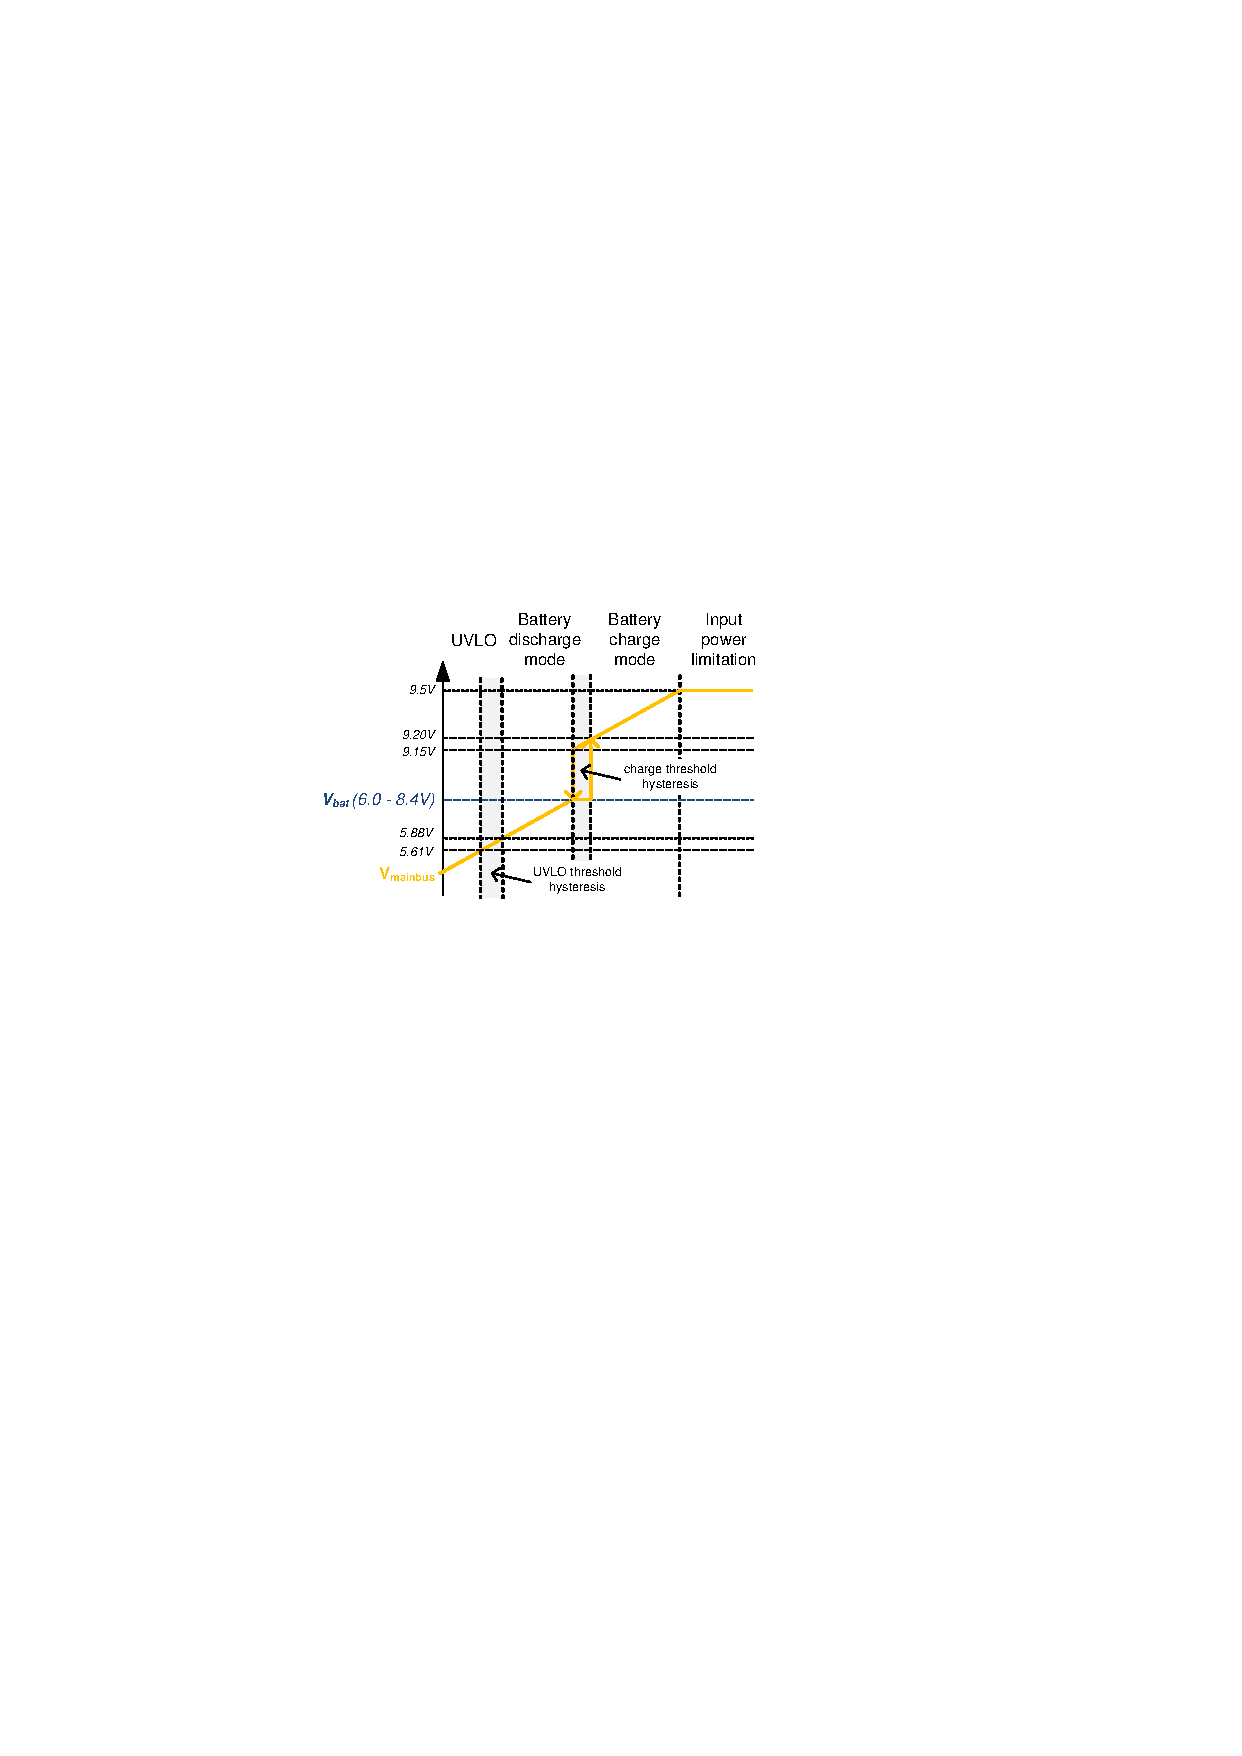
\includegraphics[width=0.8\textwidth]{figures/fig_CDR_SAR_ModeTransition}
\caption{Different SAR operation modes as function of mainbus voltage}
\label{fig:SAR_ModeTransition}
\end{figure}%
%
%
\subsection{5V Regulator}
To provide a regulated $5\,V$ supply for the on-board computer and payloads, a \textit{MIC29300-5} \ac{LDO} regulator is selected. A $2\,A$ resettable \ac{PTC} fuse is added to protect the loads from excessive currents and to protect the battery in case of a payload short-circuit failure.
%
\subsection{Complete Electrical Power System Diagram}
%
The complete \ac{EPS} diagram is shown in Figure \ref{fig:EPS_diagram_detailed}. Two $17\,A$ fuses are added in front of the motors, to protect the battery from a motor short-circuit failure.
%
\begin{sidewaysfigure}
\centering
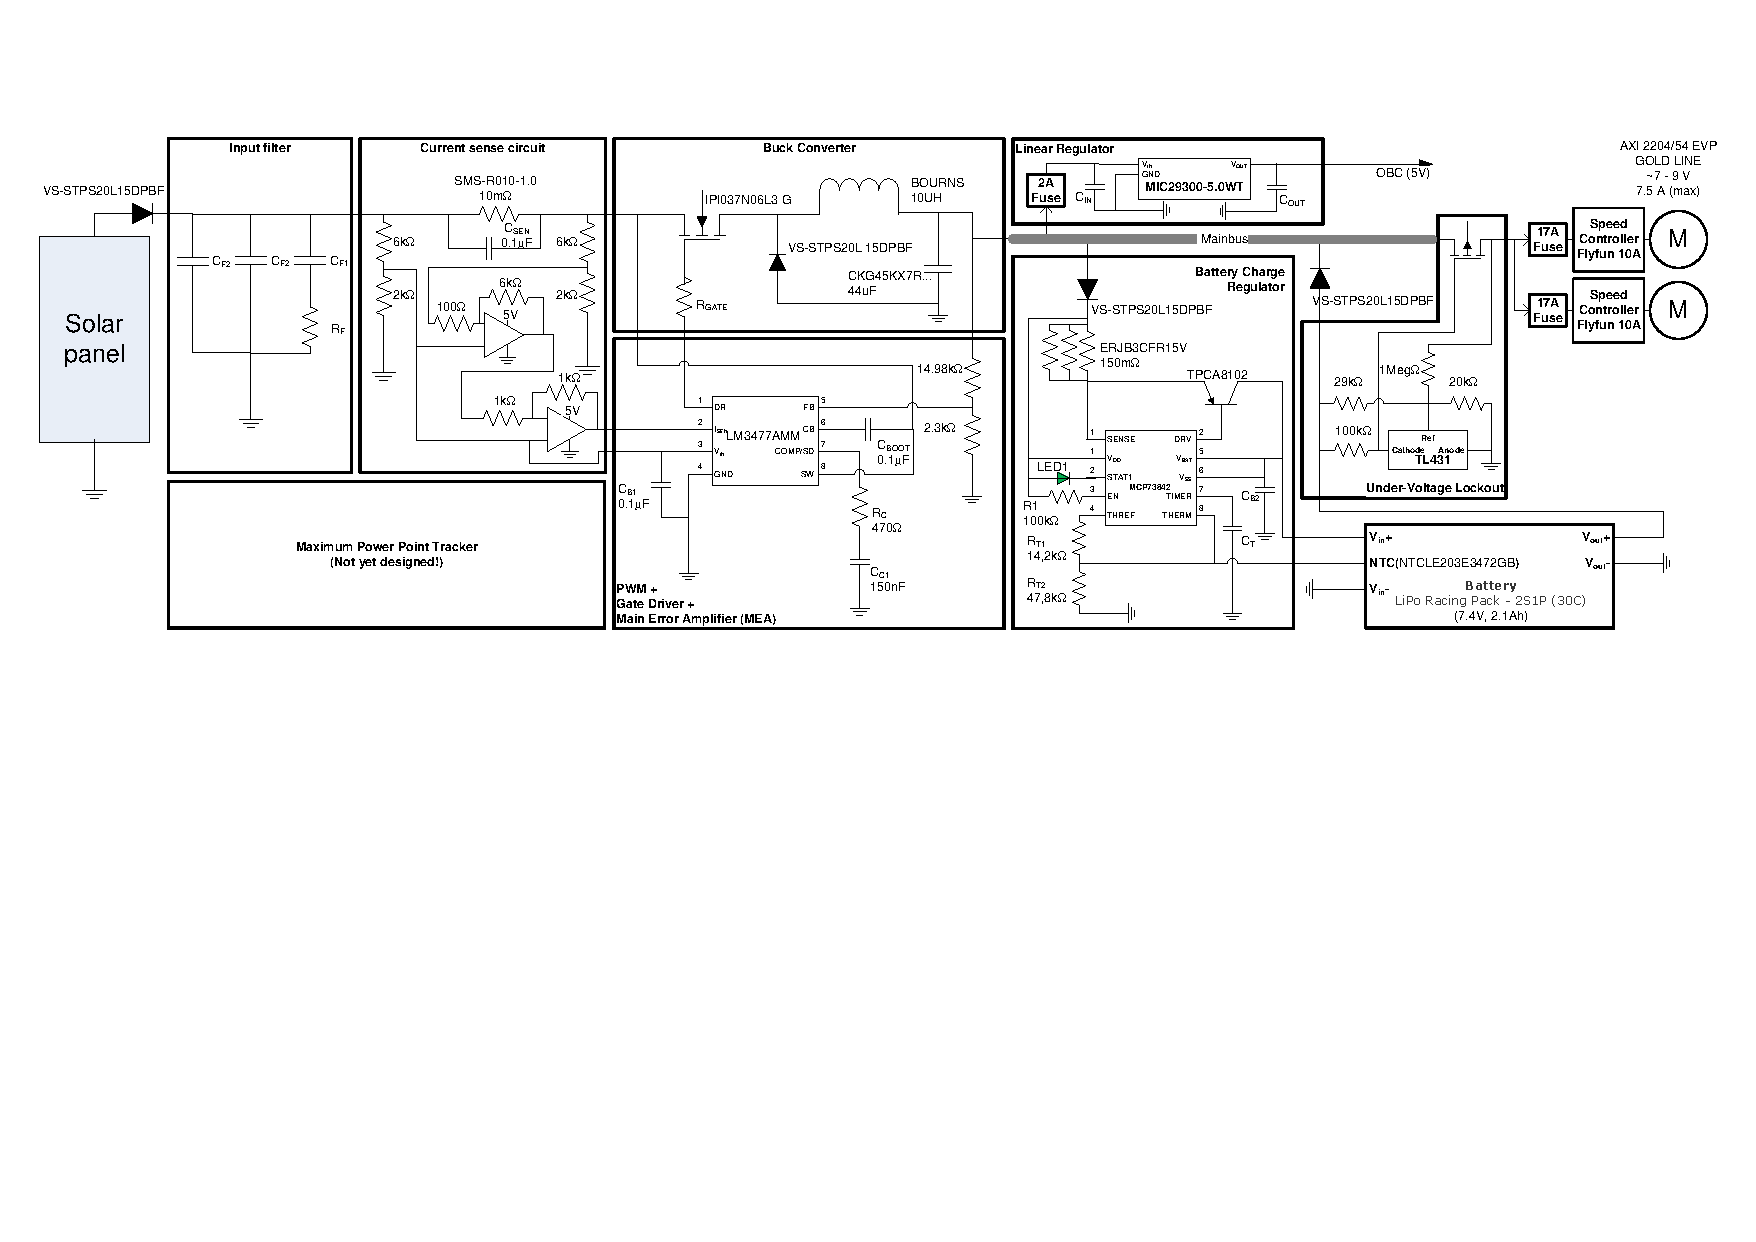
\includegraphics[width=\textwidth]{figures/fig_CDR_EPSdiagram_detailed}
\caption{EPS detailed block diagram}
\label{fig:EPS_diagram_detailed}
\end{sidewaysfigure}

%
\subsection{External Interfaces}
%
The interfaces of the \ac{EPS} external are listed in table \ref{tab:external_interfaces}.
%
\begin{table}[H]
\centering
\caption{External interfaces}
\label{tab:external_interfaces}
\begin{tabular}{m{0.3\textwidth}m{0.15\textwidth}m{0.45\textwidth}}
\hline
\textbf{External interface} & \textbf{Type} & \textbf{Implementation}\\
\hline
Solar cells mounting & Mechanical & \ac{TBD} (possibly using \ac{PSA})\\[2mm]
Power electronics mounting & Mechanical & Mounted on a \ac{PCB} which sits in the cargo bay, attached with screws\\[2mm]
Battery mounting & Mechanical & Mounted in cargo bay with strips or Velcro. Thermal insulation with Styrofoam or similar material should be added to protect against cold temperatures.\\[2mm]
\ac{EPS} telemetry & Electrical & Analog signals to Microcontroller. Electrical connector interface still remains \ac{TBD}\\[2mm]
\ac{EPS} telecommands & Electrical & \ac{TBD}\\[2mm]
Output voltages & Electrical & $6.0-9.5\,V$ (unregulated) and $5.0\,V$(regulated)\\[2mm]
\hline
\end{tabular}
\end{table}
%
%
\subsection{Telemetry and Telecommands}
The suggested \ac{EPS} telemetries are listed in Table \ref{tab:Telemetry} and the suggest telecommands in Table \ref{tab:Telecommands}. Not all telemetries or the telecommands are part of the initial \ac{EPS} design and will only be implemented if time and resources allow it.
\\
\\
The exact electrical configuration and interface connectors still remains to be designed.
%
\begin{table}[H]
\centering
\caption{Telemetry}
\label{tab:Telemetry}
%\begin{minipage}{\textwidth}
\begin{tabular}{|p{0.29\textwidth}p{0.13\textwidth}p{0.13\textwidth}p{0.35\textwidth}|}
\hline
\textbf{Telemetry} & \textbf{Data rate} & \textbf{Data size} & \textbf{Data range}\\
\hline
Battery voltage & Every 5 sec & 2 bytes & \ac{TBD}\\
\hline
Battery temperature & Every 5 sec & 2 bytes & \ac{TBD}\\
\hline
BCR status & Every 5 sec & 1 byte & high($5\,V$), low($0\,V$) and $1\,Hz\;50\%$ duty cycle ripple\footnote{for explanation of the different status indications, look in the \ac{BCR} \ac{IC} datasheet}\\
\hline
\ac{UVLO} status & Every 5 sec & 1 byte &  $0\,V$(nominal operation), $5\,V$(under-voltage lock-out)\\
\hline
Mainbus voltage & Every 5 sec & 2 bytes & \ac{TBD}\\
\hline
Solar array temperature & Every 5 sec & 2 bytes & \ac{TBD}\\
\hline
Solar array voltage & Every 1 sec & 2 bytes & \ac{TBD}\\
\hline
\end{tabular}
\end{table}
%
\begin{table}[H]
\centering
\caption{Telecommands}
\label{tab:Telecommands}
%\begin{minipage}{\textwidth}
\begin{tabular}{|p{0.25\textwidth}p{0.25\textwidth}p{0.45\textwidth}|}
\hline
\textbf{Telecommand} & \textbf{Command format} & \textbf{Description}\\
\hline
Battery charge inhibit & \ac{TBD} & Battery charging can be remotely terminated in case of battery anomalies\\
\hline
Solar array voltage set & \ac{TBD} & When \ac{MPPT} is running, the solar array operating voltage can manually be set to mitigate any malfunction in the \ac{MPPT} algorithm\\
\hline
\end{tabular}
\end{table}

\section{Test and Verification of Design}
\label{sec:test_verification}
This section describes the various design models used to develop the \ac{EPS} along with the expected functional test to be executed.
%
\subsection{EPS Design Models}
%
\subsubsection{EPS PSpice Simulations}
A transient PSpice simulation model of the whole \ac{EPS} is currently being implemented. The completed PSpice models are shown in Appendix \ref{app:EPS_PSpice}. These will help in the design and testing of the regulator performance and system stability during transient loading as well as the interactions between the different circuits.
\\
\\
In future, it is desired also to implement transient PSpice models for the solar array\cite{Castaner}, \ac{MPPTU}, battery\cite{gold}, motors and \ac{BCR}.
%
\subsubsection{EPS Development Model}
An \ac{EPS} \ac{DM} is currently being build as seen in Figure \ref{fig:EPSprototype}. The prototype \ac{PCB} is realized using self-made "mini-mount" \ac{PCB} pads as shown in Appendix \ref{app:EPS_mini-mount}. These pads are attached, using a simple glue roller, on a complete copper ground plane. This design approach allows a compact layout which reduces parasitic effects. Also any \ac{IC} package can be supported and parts can easily be moved around if the design changes.
%
\begin{figure}[H]
\centering
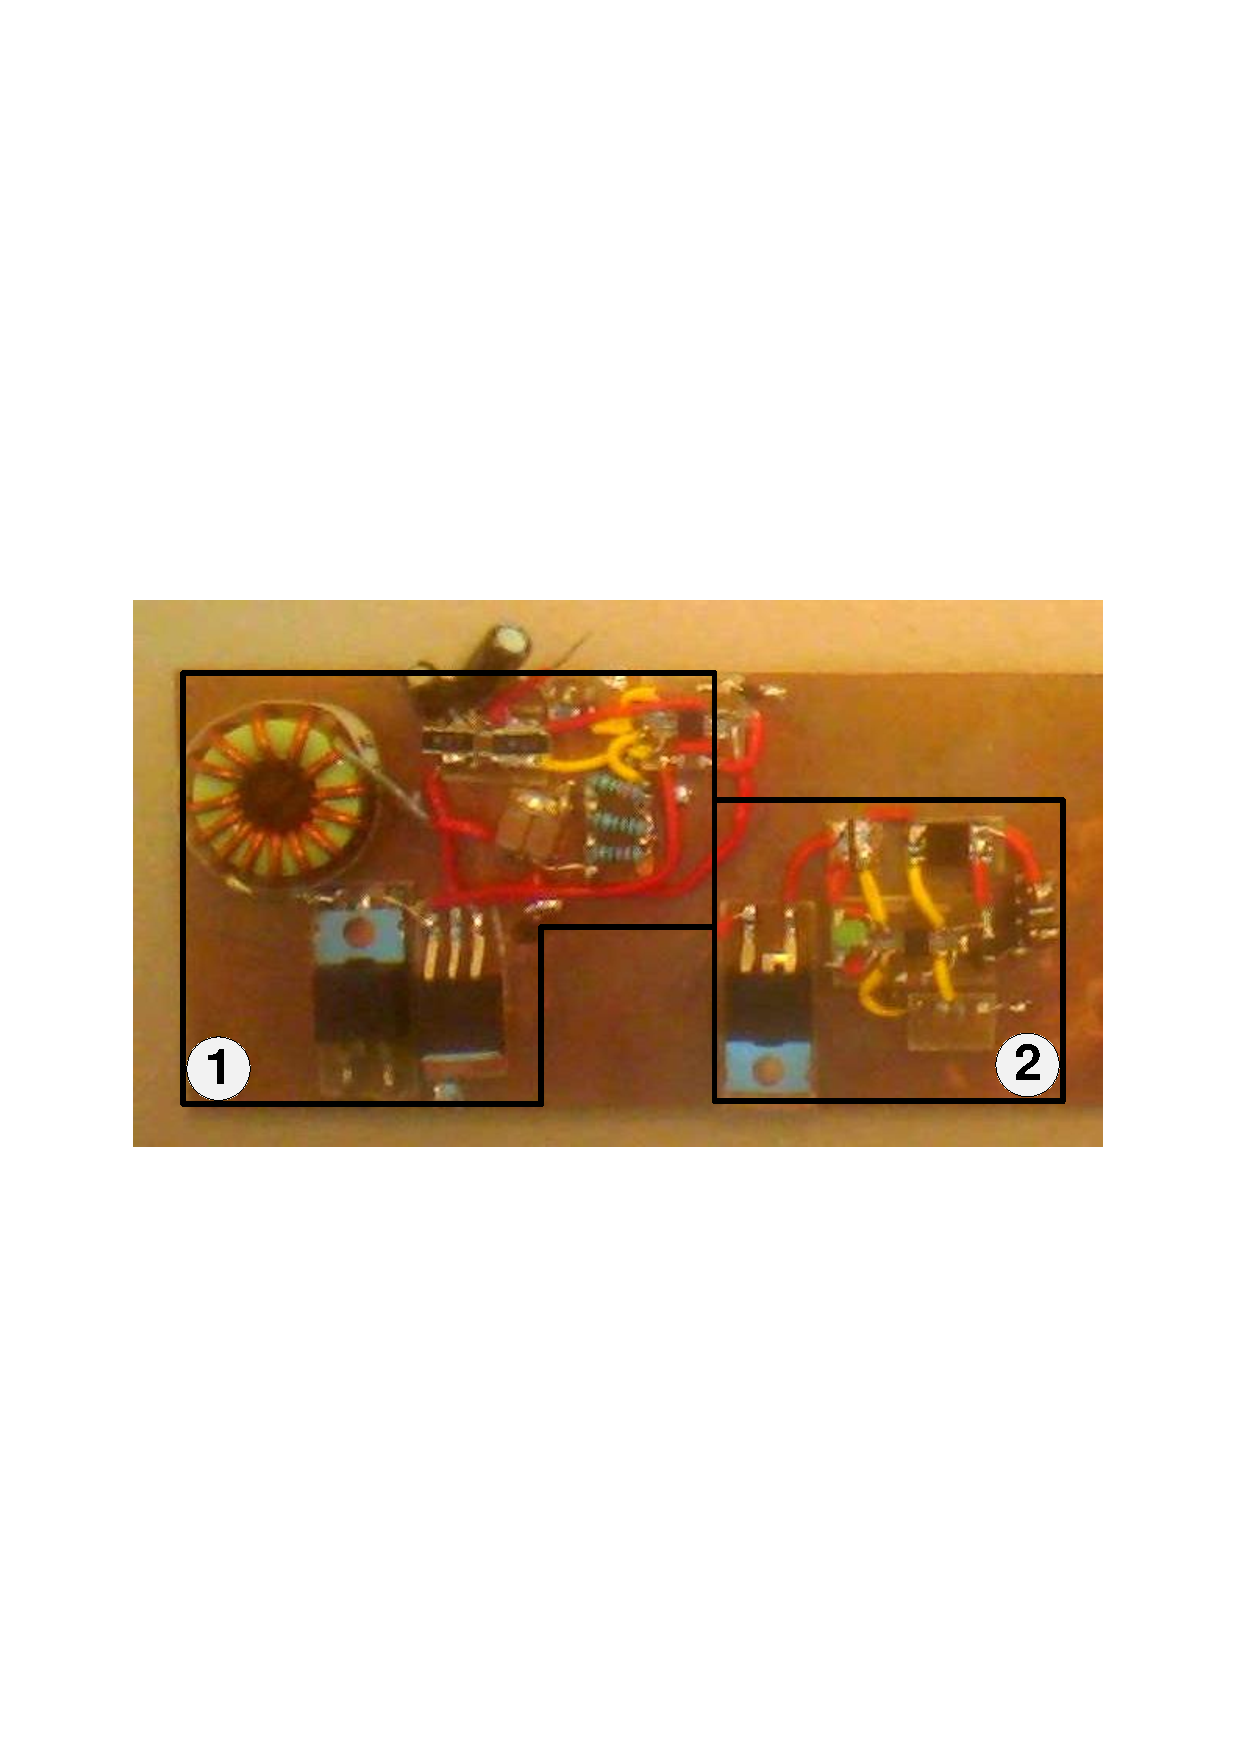
\includegraphics[width=0.8\textwidth]{figures/fig_CDR_EPSprototype}
\caption[EPS prototype]{EPS prototype - \textbf{1}: SAR, \textbf{2}: BCR}
\label{fig:EPSprototype}
\end{figure}
%
\subsubsection*{Development Model Status}
The \ac{SAR} is working but shows signs of \ac{CM} instability which is expected to be caused by the missing current sense amplifier circuit and input filter. Development progress is currently awaiting delivery of components.
\\
\\
The \ac{BCR} is also working however excessive heating of the MOSFET was experienced. A new part rated for higher power dissipation has been selected and is currently awaiting delivery.
%
\subsubsection{EPS Flight Model}
If time allows, a dedicated \ac{FM} will be build, using a custom designed \ac{PCB} schematic layout. An optimized \ac{PCB} layout will minimize the system mass and size while maximizing the efficiency and system robustness.
%
\subsection{EPS Test Program}
Table \ref{tab:test_program} lists all necessary and desired test of the EPS. Priority "1" tests are all required while priority "2" tests will only be realized if time and resources allow it.
%
\begin{center}
\begin{longtable}[H]{p{0.15\textwidth}p{0.3\textwidth}p{0.45\textwidth}r}
\caption{Test program}\\
\label{tab:test_program}\\[-0.5cm]
\hline
\textbf{Subsystem} & \textbf{Condition/Mode} & \textbf{Test Description} & \textbf{Pri.}\\
\hline
\ac{SAR} & Mainbus voltage limitation & With more input power than load power, \ac{SAR} must be able to maintain a stable $9.5\,V$ output voltage also during transient loading & 1\\
- & Maximum power handling & With an input and load power slightly above the maximum expected solar array power, no \ac{SAR} components must overheat or otherwise malfunction & 1 \\
- & \ac{MPPT} & \ac{TBD} & 2\\
- & Mode transitions & \ac{SAR} must be able to change between \ac{MPPT}, battery charge and discharge mode without loosing mainbus voltage regulation or causing other malfunctions & 2\\
- & Feedback loop stability & Regulator bandwidth, gain- and phase margins should be measured with a Network Analyzer & 2\\
- & \ac{EMC} & Electromagnetic emissions should be measured with a Spectrum Analyzer, especially with concerns to the telecommunication systems & 2\\
\hline
\ac{BCR} & \ac{CC} and trickle charging & \ac{CC} charge at $2.4\,A$ and trickle charge mode entered when battery voltage reaches $8.4\,V$ should be verified & 1\\
- & Charge inhibit at high/low temperatures & While battery is charging, battery thermistor is heated/cooled in thermal oven/fridge to slightly above/below the specified temperature limits and charging should be terminated & 1\\
\hline
\ac{UVLO} & Power cut-off and recovery & Reducing input voltage below calculated threshold voltage should open switch and switch should close again when input voltage is increased above the threshold & 1\\
\hline
Battery & Dynamic model & Test approach is described in \cite{chen} & 2\\
\hline
Solar cell & I-V specifications & short-circuit current, open-circuit voltage, current and voltage at the \ac{MPP} should be determined from an irradiance test & 2\\
- & Temperature coefficients & Solar cell temperature coefficients should be determined be measuring the I-V characteristics at different temperatures within the expected temperature interval & 2\\
\hline
Fuses & Temperature variation & The \ac{PTC} resettable fuses should be tested at nominal, minimum and maximum expected temperatures to verify acceptable functionality & 1\\
\hline
\end{longtable}
\end{center}
%

\section{Resources and Scheduling}
\label{sec:resources_scheduling}

\subsection{Main Tasks}

TBD...

%The main tasks, to implement the proposed \ac{EPS} design, are listed in table \ref{tab:main_tasks}.
%
%\begin{table}[H]
%\centering
%\caption{Main \ac{EPS} design and implementation tasks}
%\label{tab:main_tasks}
%\begin{minipage}{\textwidth}
%\centering
%\begin{tabular}{|p{0.05\textwidth}|p{0.5\textwidth}|p{0.15\textwidth}|p{0.2\textwidth}|}
%\hline
%\textbf{No.} & \textbf{Task} & \textbf{Duration [days]}\footnote{1 day = 8 effective working hours} & \textbf{Dependence (finish to start)}\\
%\hline
%1 & Design DC-DC regulator & 3 & - \\
%2 & PSpice regulator simulation & 5 & 1 \\
%3 & Order components and produce mini-mount patches\footnote{small pieces of PCB, with sticky bottom, very suitable for high frequency circuit prototyping} & 1 & 1, 2\\
%4 & Assemble solar cells & 3 & 1, 3\\
%5 & Design battery regulation and protection circuits & 3 & 1\\
%6 & Build and test battery circuits & 2 & 3, 5\\
%7 & Build prototype regulator (without MPPT) & 3 & 1, 3\\
%8 & Test prototype regulator (without MPPT) & 3 & 1, 2, 7\\
%9 & Design and build MPPT & 5 & 7\\
%10 & Test MPPT & 2 & 9\\
%11 & Design custom PCB layout & 2 & 1, 5, 9\\
%12 & Manufacture PCB and mount components & 3 & 11\\
%\hline
%\end{tabular}\par
%\vspace{-0.75\skip\footins}
%\renewcommand{\footnoterule}{}
%\end{minipage}
%\end{table}

\subsection{Parts List and Costs}
Table \ref{tab:parts_list} lists all ordered \ac{EPS} parts (including one order which is expected to be placed in the near future). The calculated costs does not including invoicing or shipping costs.
%
%
\begin{center}
\begin{longtable}[H]
{p{0.4\textwidth}p{0.25\textwidth}p{0.12\textwidth}rc}
\caption{Parts list}\\
\label{tab:parts_list}\\[-0.5cm]
\hline
\textbf{Part} & \textbf{Part Name} & \textbf{Supplier} & \textbf{Cost\footnotemark[1]} & \textbf{Qty.}\\
\hline
\endhead
\footnotetext[1]{Unit price in SEK. Actual price may differ due to currency variations}
SAR current sense resistor & FCSL110R010FER & Farnell(US) & $31.52$ & 2\\
SAR power diode & MBR3050CT & Farnell & $9.24$ & 3\\
SAR power MOSFET & IPI037N06L3 G & Farnell & $19.32$ & 4\\
SAR mainbus capacitor & CKG45NX5R1C226M & Farnell & $38.72$ & 4\\
PWM, MEA and MOSFET driver & LM3477AMM & Farnell & $16.37$ & 5\\
SAR inductor & 2101-H-RC & Farnell(US) & $25.13$ & 2\\
\acp{PCB} & CIF - AA15 & Farnell & $67.42$ & 4\\
Battery(obsolete) & PA-L60 & Farnell & $294.28$ & 2\\
Battery & LiPo Racing Pack 2S1P & Ansmann & N/A\footnotemark[2] & 1\\
\footnotetext[2]{Part was supplied by previous Spacemasters}
Reverse protection diode & VS-STPS20L15DPBF & Farnell & $24.56$ & 6\\
BCR & MCP73842-840I/UN & Farnell & $13.61$ & 2\\
BCR Transistor(obsolete) & TPCA8102(TE12L,Q) & Farnell & $28.5$ & 2\\
Current limit \ac{BJT}(obsolete) & 2STN2540 & Farnell & $7.84$ & 5\\
Current limit MOSFET(obsolete) & IRLML6401PBF & Farnell & $6.41$ & 2\\
BCR current sense resistor & ERJB3CFR15V & Farnell & $1.97$ & 5\\
Current limit sense resistor(obsolete) & ERJB2BFR33V & Farnell & $4.83$ & 5\\
Current limit sense resistor 2(obsolete) & ERJA1BJR27U & Farnell & $5.30$ & 5\\
Power limit \ac{BJT}(obsolete) & STN888 & Farnell & $5.49$ & 5\\
Solar cell & RC7.2-75(PSA) & Eco Power Shop & $230.08$ & 2\\
Solar cell(obsolete) & MC-SP0.8-NF-GCS & Farnell & $66.51$ & 2\\
\ac{LDO} regulator & MIC29300-5.0WT & Farnell & $74.85$ & 2\\
Current sense OpAmp & LTC6362CMS8\# PBF & Farnell & $32.31$ & 2\\
Thermistor & NTCLE203E3472GB0 & Farnell & $8.64$ & 5\\
Motor fuses & RGEF1000 & Farnell & $6.46$ & 5\\
\ac{LDO} regulator fuses & MC36248 & Farnell & $1.41$ & 5\\
\ac{BCR} MOSFET & SUP75P03-07-E3 & Farnell & $31.51$ & 2\\
\ac{UVLO} linear shunt regulator & TL431AILPME3 & Farnell & $1.36$ & 5\\
\ac{UVLO} MOSFET & SUP75P03-07-E3 & Farnell & $31.51$ & 2\\
\hline\hline
Total cost & & & 2707.6 & \\
\hline
\end{longtable}
\end{center}
%
%
\subsection{Electrical Ground Support Equipment}
The \ac{EGSE} in Table \ref{tab:EGSE} is mainly required for testing of the \ac{EPS}.
%
\begin{table}[H]
\centering
\caption{Required EGSE}
\label{tab:EGSE}
\begin{tabular}{|p{0.35\textwidth}p{0.55\textwidth}|}
\hline
\textbf{Instrument} & \textbf{Required Specifications}\\
\hline
Network Analyzer & Up to about $\sim 1\,MHz$\\
Spectrum Analyzer & \ac{TBD}\\
Power supply & $75\,W$ output power at $\sim 15\,V$\\
Heating and cooling chamber(s) & $-20^{\circ}C$ to $+45^{\circ}C$ and allow small wires to be pulled through chamber\\
\hline
\end{tabular}
\end{table}
%
%
\subsection{Mechanical Ground Support Equipment}
The required \ac{MGSE} is mainly for \ac{PCB} manufacturing, i.e. UV light source, photo developing facility, etching facility, drills, cutters etc.